\documentclass[letterpaper,12pt,fleqn]{article}
\usepackage{matharticle}
\usepackage{siunitx}
\usepackage{pgfplots}
\pgfplotsset{compat=1.14}
\pagestyle{plain}
\begin{document}

\begin{center}
\Large Math-8 Final Exam
\end{center}

\vspace{0.5in}

Name: \rule{4in}{1pt}

\vspace{0.5in}

This exam is closed book and notes, except for a two-sided $3\times 5''$ index card of
notes. You may also use a graphing calculator; however, no other electronics are allowed.
Show all work in an organized fashion; there is no credit for guessed answers or work
that I cannot follow or doesn't appear to lead to your answers. All answers should be in
exact values unless you are specifically asked for an approximate value.

\vspace{0.5in}

\begin{enumerate}
\item Consider the following graph of the function $y=f(x)$:

  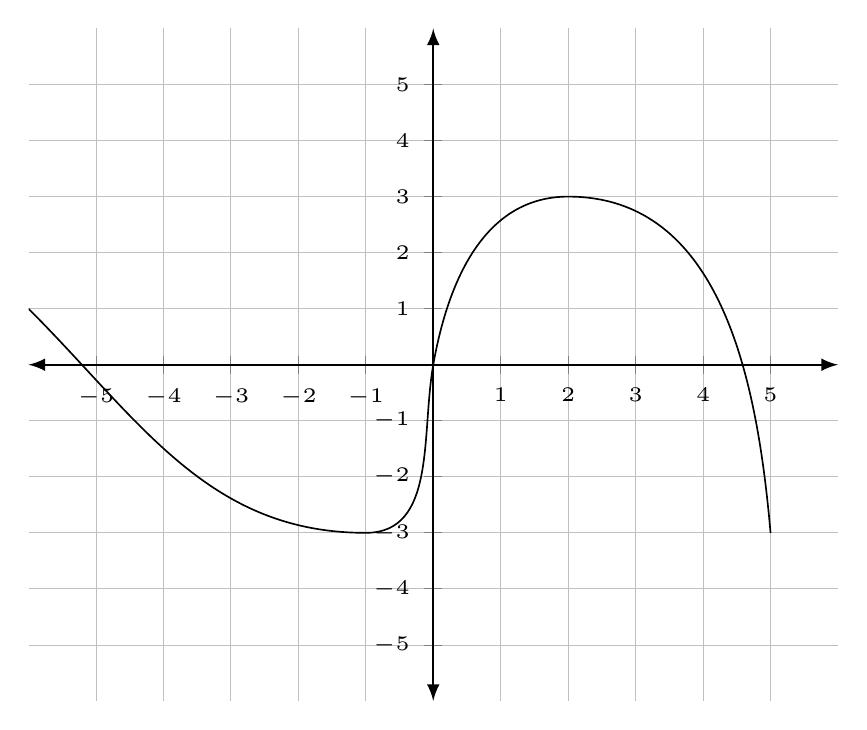
\begin{tikzpicture}[scale=1.5]
    \begin{axis}[
        xmin=-6,xmax=6,
        ymin=-6,ymax=6,
        grid=both,
        grid style={line width=.1pt, draw=gray!10},
        major grid style={line width=.2pt,draw=gray!50},
        axis lines=middle,
        axis line style={latex-latex},
        xtick={-5,-4,-3,-2,-1,0,1,2,3,4,5},
        ytick={-5,-4,-3,-2,-1,0,1,2,3,4,5},
        ticklabel style={font=\tiny},
      ]
      \draw (-6,1) to [out=-45,in=180] (-1,-3);
      \draw (-1,-3) to [out=0,in=-100] (0,0);
      \draw (0,0) to [out=80,in=180] (2,3);
      \draw (2,3) to [out=0,in=95] (5,-3);
    \end{axis}
  \end{tikzpicture}

  Assume that $f(x)\to\infty$ as $x\to-\infty$ and $f(x)\to-\infty$ as $x\to\infty$.
  \begin{enumerate}
  \item Where is the function increasing (in interval notation)?

    \vspace{0.5in}
    
  \item Where is the function decreasing (in interval notation)?
  \end{enumerate}

  \newpage

\item Circle the polynomial function that best matches the following graph:

  \begin{minipage}{\textwidth}
    \setlength{\leftskip}{1in}
    \begin{tikzpicture}
      \draw [<->] (-3,0) -- (3,0);
      \draw [<->] (0,-3) -- (0,3);
      \draw [smooth,domain=-1.4:1.4] plot ({\x},{(\x)^4-1});
    \end{tikzpicture}
  \end{minipage}

  \[\begin{array}{clclclcl}
  f(x)=(x-1)^4 & \quad & f(x)=(x+1)^4 & \quad & f(x)=x^4+1 & \quad & f(x)=x^4-1 \\
  \\
  f(x)=(x-1)^5 & \quad & f(x)=(x+1)^5 & \quad & f(x)=x^5+1 & \quad & f(x)=x^5-1
  \end{array}\]

\item Evaluate the following expression without using a calculator:
  \[\log_2(8)=\]

\item Consider the following graph of the function $y=f(x)$:

  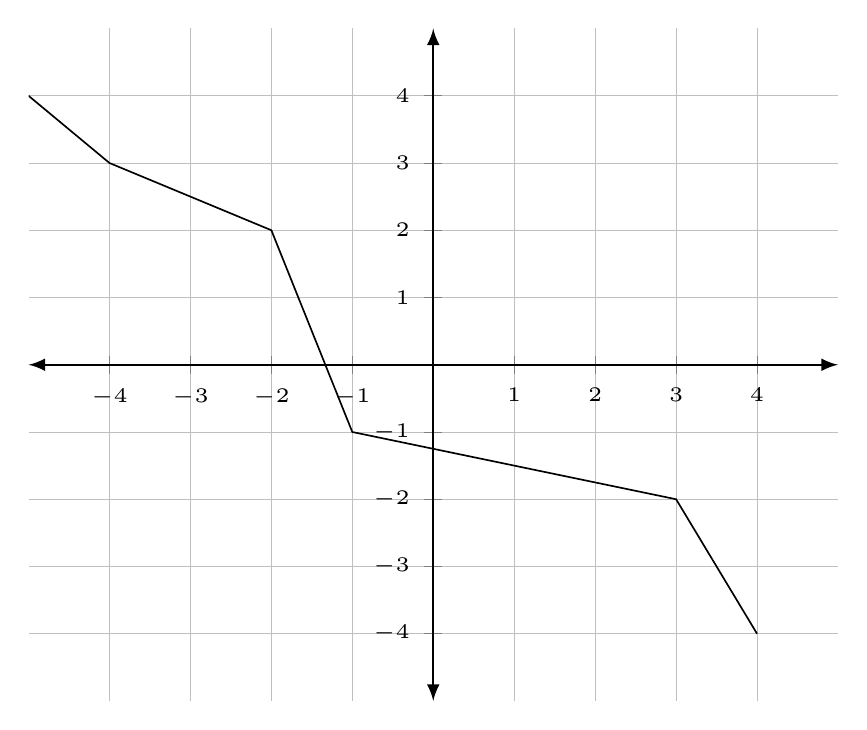
\begin{tikzpicture}[scale=1.5]
    \begin{axis}[
        xmin=-5,xmax=5,
        ymin=-5,ymax=5,
        grid=both,
        grid style={line width=.1pt, draw=gray!10},
        major grid style={line width=.2pt,draw=gray!50},
        axis lines=middle,
        axis line style={latex-latex},
        xtick={-4,-3,-2,-1,0,1,2,3,4},
        ytick={-4,-3,-2,-1,0,1,2,3,4},
        ticklabel style={font=\tiny},
      ]
      \draw (-5,4) -- (-4,3) -- (-2,2) -- (-1,-1) -- (3,-2) -- (4,-4);
      \end{axis}
  \end{tikzpicture}

  Find the following value:
  \[f^{-1}(3)=\]

\item Solve for $x$. Your answer must be in interval notation.
  \[\abs{2x-1}+3\le6\]

  \vspace{4in}

\item Let $f(x)=\sqrt[3]{x+5}$ and $g(x)=x^2-4$. Determine the following composite
  function (you do not need to simplify):
  \[(f\circ g)(x)=\]

\item Solve for $x$ using the quadratic formula. Be sure to leave your answer in exact
  form:
  \[5x=13-3x^2\]

  \newpage

\item Divide $x^3-5x^2+2x-7$ by $x^2+3x-4$. Write your final answer in division
  algorithm form.

  \newpage

\item Consider the following equation of a circle:
  \[x^2-4x+y^2-9x+1=0\]
  \begin{enumerate}
  \item Convert the general form to standard form.

    \vspace{3in}

  \item What are the coordinates of the center and the length of the radius?

    \vspace{1in}

  \end{enumerate}

\item Compute and simplify completely the difference quotient for $f(x)=3x-x^2$.

  \newpage

\item Consider the relation $y^2+3xy-2x=36$.
  \begin{enumerate}
  \item Determine all $x$-intercepts (if any). Remember to state as points.

    \vspace{1.5in}
    
  \item Determine all $y$-intercepts (if any). Remember to state as points.
    
    \vspace{1.5in}
    
  \end{enumerate}

\item Determine the equation of the line that is perpendicular and through the midpoint
  of the line connecting the points $(-2,5)$ and $(7,1)$. Your answer must be in
  slope-intercept form.

  \newpage

\item Katya deposits $\$1000$ in an interest-bearing account. The amount of money in
  her account after $t$ years is given by:
  \[A=1000e^{0.05t}\]
  \begin{enumerate}
  \item What is the compounding period?

    \vspace{1in}

  \item What is the interest rate (with units)?
    
    \vspace{1in}

  \item What is the account balance after 2 years?

    \vspace{2in}

  \item How long does it take for the account balance to reach $\$2500$? Round your
    answer to one decimal point and don't forget to state the units.

    \vspace{3in}

  \end{enumerate}

  \newpage

\item Solve for $x$:
  \[x-\frac{10}{x+1}=2\]

  \vspace{2.5in}

\item Consider the parabolic function:
  \[f(x)=x^2-6x-5\]
  \begin{enumerate}
  \item Convert the general form to standard form.

    \vspace{2.5in}

  \item What are the coordinates of the vertex?

    \newpage

  \item What are the $x$-intercepts (if any)?

    \vspace{2in}

  \item What are the $y$-intercepts (if any)?

    \vspace{2in}

  \item Sketch the graph. You must label the vertex and all intercepts.

    \vspace{3in}

  \item State the domain and range in interval notation.
    
  \end{enumerate}

  \newpage

\item Consider the following expression:
  \[\ln\frac{x^3}{13\sqrt{y}}\]
  Expand completely using the properties of logs.

  \vspace{3in}

\item Let $f(x)=5x-7$
  \begin{enumerate}
  \item Find $g(x)=f^{-1}(x)$

    \vspace{2in}
    
  \item Prove that $f$ and $g$ are inverses.
    
    \vspace{3in}

  \end{enumerate}

\item Find the domain (in interval notation) of the function $f(x)=\sqrt{x^2-4x-5}$.

  \vspace{4in}

\item Consider the following function:
  \[f(x)=1-\sqrt{x+2}\]
  \begin{enumerate}
  \item List the standard function and the transformations in the order that they are
    applied.
    \begin{enumerate}
      \item
      \item
      \item
      \item
    \end{enumerate}

  \item Determine the $x$-intercepts (if any).

    \newpage

  \item Determine the $y$-intercepts (if any).
    
    \vspace{1in}

  \item Sketch the graph. You must label all important points.

    \vspace{4in}

  \end{enumerate}
  
  \newpage

\item Consider the following polynomial function:
  \[f(x)=x^3-4x^2+x+6\]
  \begin{enumerate}
  \item Factor completely. For full credit you must show how you determine the
    candidate zeros, how you selected the actual zeros, and how you use long (or
    synthetic) division.

    \newpage

  \item Sketch the graph. For full credit you must label all intercepts and state how
    you determined the behavior at each zero using either a sign table or multiplicity.

    \vspace{5in}

  \item Using your calculator, determine all minima and maxima (there should be two).
    
  \end{enumerate}
\end{enumerate}

\end{document}
